\documentclass[english,11pt,a4paper]{article}
%\usepackage{fullpage}
\usepackage[margin=2cm]{geometry}

\usepackage[T1]{fontenc}



%dodatni paketki:
\usepackage{graphicx}
\usepackage{amsmath,amsfonts,amsthm} %matematicni paket
\usepackage{color} % omogoča barvno pisanje
\usepackage[utf8]
{inputenc}
\usepackage[english]{babel} % slovenski jezik/hyphenation
\usepackage{hyperref} %naredi vse povezave rečerenc, kazala,...
\numberwithin{equation}{section} % Number equations within sections (i.e. 1.1, 1.2, 2.1, 2.2 instead of 1, 2, 3, 4)
\numberwithin{figure}{section} % Number figures within sections (i.e. 1.1, 1.2, 2.1, 2.2 instead of 1, 2, 3, 4)
\numberwithin{table}{section} % Number tables within sections (i.e. 1.1, 1.2, 2.1, 2.2 instead of 1, 2, 3, 4)
\usepackage{eurosym} %za znak €
\usepackage{url}



\usepackage{mathrsfs}
%\usepackage{mathabx} % za kemisjke smeri in naslednje 3 vstrice
\catcode`_=12
\begingroup\lccode`~=`_\lowercase{\endgroup\let~\sb}
\mathcode`_="8000


\usepackage[margin=2cm]{geometry}




\begin{document}
\begin{titlepage}

\newcommand{\HRule}{\rule{\linewidth}{0.5mm}} % Defines a new command for the horizontal lines, change thickness here

\center % Center everything on the page

%----------------------------------------------------------------------------------------
%	LOGO
%----------------------------------------------------------------------------------------

%\includegraphics{Logo}\\[1cm] % Include a department/university logo - this will require the graphicx package
 
%----------------------------------------------------------------------------------------


\includegraphics[width=2cm]{slike/aaa}\\[0.5cm]
 
%----------------------------------------------------------------------------------------
%	NASLOV DELA
%----------------------------------------------------------------------------------------
\textit{Univerity of Ljubljani}\\
\textit{Faculty of {\color{red}{Mathematics and Physics}}}\\[0.5cm]

\emph{Department of Physics}\\[0.5cm] % Oddelek za fiziko


%----------------------------------------------------------------------------------------
%	TITLE SECTION
%--------------------------------------------------------------------------------------
\HRule \\[0.4cm]
\huge {\bfseries Spectroscopy in terahertz range}\\[0.4cm] % NASLOV SEMINARJA
\HRule \\[0.5cm] 

 \Large \emph{Seminar 1a}\\[1cm] % SEMINASKO DELO
 
%----------------------------------------------------------------------------------------
%	AUTHOR SECTION
%----------------------------------------------------------------------------------------


\Large \emph{Author:}\\
Klemen \textsc{Rahne}\\[1cm]

\Large \emph{Mentor:}\\
prof. dr. Marko \textsc{Zgonik}\\[1cm]




% If you don't want a supervisor, uncomment the two lines below and remove the section above

%----------------------------------------------------------------------------------------
%	DATUM
%----------------------------------------------------------------------------------------

{\large \today } \\[0.5cm] % Date, change the \today to a set date if you want to be precise

	

\vfill
\begin{center}
\textsc {Abstract}\\[0.5cm]

Nek povzetek, bla bla bala, hahaha, tekx+st, nekaj pišem samo da dela.

\end{center}
\end{titlepage}


%----------------------------------------------------------------------------------------
%	KAZALO
%----------------------------------------------------------------------------------------

\tableofcontents

%----------------------------------------------------------------------------------------
%	ZAČETEK TEKSTA
%----------------------------------------------------------------------------------------


\section{Introduction}

One of last region of electromagnetic radiation to be researched was terahertz range. Major problem in study of terahertz radiation was lack of good sources and detectors in this range of electromagnetic radiation. In last decades laser technologies unlocked new events in materials causing generating radiation in terahertz radiation. With further researches in terahertz region terahertz spectroscopy showed some encouraging new technologies for detection of explosives, counterfeit drugs or skin cancer.

\section{Terahertz radiation}
Terahertz radiation as prefix denotes, it has frequency with order of magnitude $12$ Hertz\textcolor{red}{Ali to OK??}. This frequency corresponds to wavelength of $300\mu m$\footnote{If this radiation is propagating in vaccum.}. With photon energy in around few $meV$, is this radiation non-ionizating and "nakazuje" in non invasize measurment (medical scnning, tehniques). As seen in diagram \ref{em-spectrum}, terahertz radiation (hereinafter THz radiation) covers gap between optical and electronical part of electromagnetum spectrum. With transistors and other components based on electronic transport we can achive upper frequancy limit of about $300GHz$, while with semiconductor lasers we can achive minimal frequency of $30THz$. Therefore we must find new \textcolor{red}{visokoizkoristkljive} tehnieques to generatee and measure THz radiation.


 
 
 
\begin{figure}[!htb]
\label{em-spectrum}
\centering
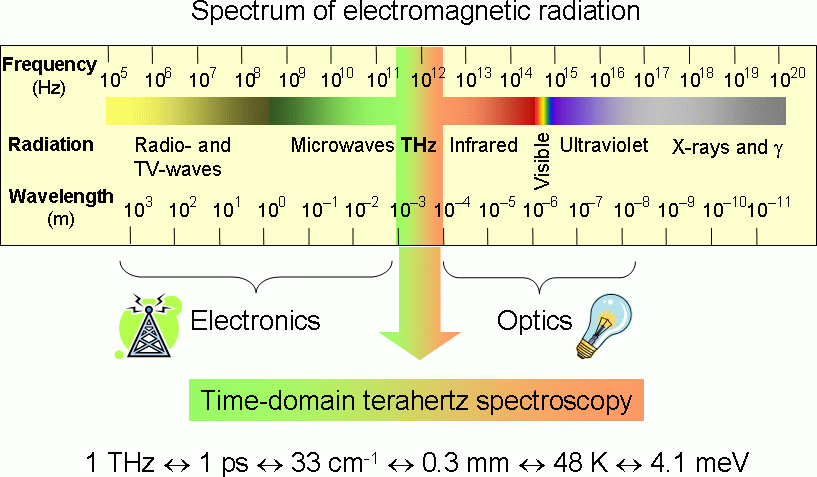
\includegraphics[scale=0.5]{slike/spectrum_b.png}
\caption{Electromagnetic radiation spectrum and position of terahertz radiation. \cite{em-spectrum}}
\end{figure}

\begin{figure}[!htb]
\label{TDS-spectrum}
\centering
\includegraphics[scale=0.5]{slike/wavefrm_b.png}
\caption{ An example of a temporal profile of electric field of a typical terahertz pulse (left panel) and its spectrum (right panel). The useful spectrum of the terahertz pulse spans over more than one decade (0.1 – 3 THz).\textcolor{red}{text je copy/past/SPREMENI!!}  \cite{em-spectrum}}
\end{figure}
%
%This frequecy area lies between electronical and optical part of electromagnetic radiation. 
% between $0.3$ and $3THz$ with corresponding wavelength from $100 \mu m$ to $1mm$. This gap lies between electronical and optical part of electromagnetical radiation.
%\section{Terahertz generation}
%
%
%\section{Tereahertz detection}
%
%The electric field of THz radiation that the probe pulse experience can be approximated as a DC bias field since the THz pulse is much longer than theprobe pulse ( 1 ps vs. 100 fs), and the whole time profile of the THz pulse can therefore be traced by measuringthe phase retardation (see eq. 2.40) using a variable delay line (VDL) to temporally delay the \cite{TTDS}
%
%



\section{Terahertz spectroscopy}




\newpage

  \begin{thebibliography}{}\addcontentsline{toc}{section}{\bibname}

  \bibitem{notes} John W. Dower {\em Readings compiled for History  21.479.}  1991.
    \bibitem{em-spectrum} http://lts.fzu.cz/en/intro.php, 20.8.2018.

  \bibitem{TTDS} Hans Christian Bakken Skjeie {\em Terahertz Time-Domain Spectroscopy} Master of Science in Electronics

  \bibitem{norman} E. H. Norman {\em Japan's emergence as a modern
  state} 1940: International Secretariat, Institute of Pacific
  Relations.

  \bibitem{fo} Bob Tadashi Wakabayashi {\em Anti-Foreignism and Western
  Learning in Early-Modern Japan} 1986: Harvard University Press.

  \end{thebibliography}


\end{document}
